\section{Лекция 4}
\subsection{Возвращение к истокам.}
Напомним, что на предыдущих лекциях мы пытались решали задачу проверки тавтологичности формулы.\\
Для проверки тавтологичности формулы мы построили специальное исчесление высказываний - формальную систему, которая основана на правиле MP \ref{def:MP} (из семантики $a,a\to b \vDash b$). Но мы сталкиваемся с одной трудностью - не ясно, с чего начинать вывод, что считать первой формулой в выводе.\\
Можно провести конструктивное доказательство тавтологичности формулы, но для него нам нужна таблица истинности. Он корректен и полон, но слишком длинный.\\
\subsection{Правило резолюции.}
\textbf{Сегодня рассмотрим доказательство тавтологичности формулы, основанное на правиле резолюции}\\
\begin{definition} \label{def:resolution} \tit{Правило резолюции:}\\
Из семантического наблюдения : $a\vee b, \neg a\vee c \vDash b\vee c$\\
Синтаксическое правило: $\frac{A\vee B,\neg A\vee C }{B\vee C}$
(Резолюции)
\end{definition}
\textbf{Вывод}\\
От противного: $b\vee c=0\Rightarrow b=0 \wedge c=0\Rightarrow a\vee b=a, \neg a\vee c=\neg a\Rightarrow a, \neg a - \text{несовместно}$\\
Приведем пример:\\
\begin{figure}[!h]
	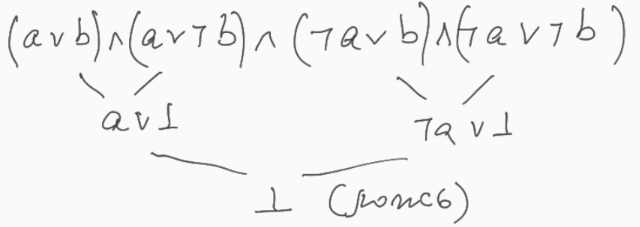
\includegraphics[width = 0.6\linewidth]{resol.png}
\end{figure}
\newline
Заметим, что особенностью метода резолюций является то, что он \textbf{проверяет невыполнимость КНФ}.
\subsection{Дизъюнкты.}
\begin{definition} \label{def:diz} \tit{Дизъюнкты - }
это дизъюнкции литералов $x, \neg x$
\end{definition}
\begin{definition} \label{def:diz} \tit{Стандартные дизъюнкты: }
\[a\vee \neg a = T\\
a\vee a = a
\]
Стандартные дизъюнкты - это множество литералов.\\
$\bot$(ложь)- пустое множество (пустой дизъюнкт).\\
Если есть множество переменных: $x_1,x_2,...,x_n$.\\
Есть литералы $D\subseteq \{x_1,...,x_n,\neg x_1,...,\neg x_n\}$ и $T$- тождественная истиность (не является множеством).
\end{definition}
\begin{definition}\label{def:dizl} \tit{Дизъюнкция литералов: }\\
\[
D_1\vee D_2= D_1 \cup D_2 \hspace{3mm} \text{или} \hspace{3mm} T,\hspace{3mm} \text{если} \hspace{3mm} x\in D_1\vee D_2, \neg x \in D_1\vee D_2
\]
\end{definition}
\subsection{Резолюции.}
Рассмотрим частный вид правила резолюции:
\[
(R)\hspace{3mm} \frac{x\vee D_1,\neg x\vee D_2 }{D_1\vee D_2}
\]
\textbf{Что, если $D_1\vee D_2=T$???}\\
Такой дизъюнкт бесполезен в доказательстве несовместимости. Тогда будем считать, что правило (R) неприменимо в данном случае.\\
\textbf{Рассмотрим, когда $D_1\vee D_2\neq T$}
Введем такое понятие, как \textbf{резолютивный вывод.}\\
\begin{definition}\label{def:resv} \tit{Резолютивный вывод из множества Г =$\{D_1,D_2,...,D_k,...\}$ дизъюнктов -  }
последовательность $D_1^{'},...,D_n^{'}$ дизъюнктов такая, что для любого члена последовательности выполняется одно из двух:
\begin{center}
$D_i^{'}\in \Gamma$\\
\textbf{или}\\
$ (R)\hspace{3mm} \frac{D_j^{'},D_k^{'} }{D_i^{'}} (j,k<i)$ \textbf{ , то есть }
$ \frac{D_j^{'}= x\vee D_j^{''} ,D_k^{'}=\neg x\vee D_k^{''} }{D_i^{'}=D_j^{''}\vee D_k^{''}}$
\end{center}
\end{definition}
Введем новое обозначение: 
\[
\Gamma \underset{(R)}{\vdash} D, \text{если D встречается в резолютивном выводе.}
\]
\begin{definition}\label{def:contrres} \tit{Опровержением множества $\Gamma$ резолюциями} будем называть $\Gamma \vdash \bot $
\end{definition}
\textbf{Корректность:}\\
\[
\Gamma \vdash \bot \Rightarrow \Gamma \vDash \bot \hspace{3mm} \textbf{(Г - несовместно)}
\]
\textbf{Доказательство корректности:}\\
От противного. Пусть $\Gamma$ совместно. $D\in \Gamma \Rightarrow D(\alpha)=1$ для некоторого $\alpha$. Индукцией по длине вывода $D_1^{'},...,D_N^{'}$ проверяем, что $D_i^{'}(\alpha)=1$. Есть два случая:
\begin{enumerate}
    \item $D_i^{'}\in \Gamma \Rightarrow D_i^{'}(\alpha)=1$
    \item $ \frac{D_j^{'}= x\vee D_j^{''} ,D_k^{'}=\neg x\vee D_k^{''} }{D_i^{'}=D_j^{''}\vee D_k^{''}} \hspace{3mm} \Rightarrow \hspace{3mm}$ 
       $ \begin{cases}
        x \vee D_j^{''}( \alpha )=1\\
        \neg x\vee D_k^{''}(\alpha)=1
        \end{cases}$
        $\Rightarrow D_i(\alpha)=(D_j^{''}\vee D_k^{''})(\alpha)=1$
        \newline
        \hspace*{90mm} $(a\vee b, \neg a\vee c \vDash b\vee c)$
\end{enumerate}
\textbf{Полнота:}
\[\Gamma \vDash \bot \Rightarrow \Gamma \vdash \bot\]
\[\text{(все, что несовместно - опровержимо)}\]
\textbf{Идея пополнения (доказательства):}\\
$\Gamma^{'}= \{D|\Gamma \vdash D\}$ (выведем все, что возможно).\\
$\bot \notin \Gamma^{'} \Rightarrow \Gamma^{'}$- совместно (контрпозиция полноты).\\
Теперь построим расширяещееся множество дизъюнктов 
\[
\Gamma_1 \subseteq \Gamma_2\subseteq ... \Gamma_k \subseteq...\subseteq \Gamma^{'}
\]
Причем $\Gamma_k$- дизъюнкты, в который входят только $x_1,...,x_k$ первые $k$ перменных.\\
Построим выполняющий набор следующим образом: $x_1=\alpha_1,x_2=\alpha_2,... $\\
Введем следующее правило:
\[
\alpha_{k+1}= 
\begin{cases}
0, \text{если нет } D\in \Gamma_{k+1} \text{ и нет дизъюнкта } D(\alpha_1 , \alpha_2 , ... \alpha_k , 0)\\
1 (T), \text{иначе}
\end{cases}
\]
Данное правило дает нам выполняющий набор. Докажем данный факт.\\
\newpage
\textbf{Доказательство:}\\
Хотим доказать, что $D\in \Gamma^{'}\Rightarrow D(\alpha)=1$. Заметим, что это равносильно тому, что $\forall n \forall D: D\in \Gamma_n \Rightarrow D(\alpha)=1$.\\
Проведем доказательство по индукции по $n$.\\
\textbf{База:} $n=1 : x\notin \Gamma^{'} \text{ или } \neg x \notin \Gamma^{'} 
\textbf{ (иначе } \bot \in \Gamma^{'})$\\
\textbf{Шаг индукции:} $\forall D \in \Gamma_k \hspace{3mm} D(\alpha)=1$ от противного.\\
$D \in \Gamma_{k+1}$ и $D(\alpha_1,...,\alpha_{k+1}=0 \leftrightarrow \alpha_{k+1} = 1$ по построению.\\
$D = \neg x_{k+1} \vee D^{'}(x_1,...,x_k)$ и $D^{'}(\alpha_1,...,\alpha_{k+1}=0$\\
\textbf{НО} существует:\\
\[\hspace{5mm} D_1 \in \Gamma_{k+1} \hspace{50mm} D_1= x_{k+1} \vee D^{''}\]
\[
D_1(\alpha_1,...,\alpha_k,0) \hspace{50mm} D^{''}(\alpha_1,...,\alpha_k)=0
\]
Применим к $D = \neg x_{k+1} \vee D^{'}(x_1,...,x_k)$ и $D_1= x_{k+1} \vee D^{''}$ применим правило резолюции. А значит получим:
\[
\frac{D_1,D}{D^{'}\vee D^{''}} \Rightarrow
\begin{cases}
D^{'}\vee D^{''} \in \Gamma_k\\
(D^{'}\vee D^{''})(\alpha)=0\\
\end{cases}
\Rightarrow \textbf{противоречие.}
\]
\subsection{Как доказывать общие формулы?}
Ранее в этой лекции мы разобрали систему доказательств тавтологичности для ДНФ.\\ Вы скажете: "Но как же? Речь шла о КНФ?".\\
А я обращу ваше внимание на следующее:
\[
\neg \textbf{ДНФ $=$ КНФ}\]
\[
\textbf{ДНФ - тавтология $\leftrightarrow \neg $ ДНФ невыполнимо $\leftrightarrow \neg$ ДНФ $\vdash \bot$ (в резолюциях)}
\]
Вернемся к насущному вопросу: как же быть с общими формулами?\\
\textbf{1 способ.} Совершенная КНФ $f: \{0,1\}^n \to \{0,1\}$\\
\[
f(x) = \underset{\alpha: f(\alpha)=0}{\bigwedge} \hspace{3mm} \bigvee\limits_{i=1}^n x_i^{\neg \alpha_i}
\]
\[
\begin{pmatrix}
  x^0= \neg x& x^{1}=x\\
  a^a=1& a^{\neg a}=0
\end{pmatrix}
\]
Но мы вновь сталкиваемся с одной важной проблемой - для построения КНФ нам нужна таблица истинности(((
\subsection{Выход есть - идея сводимости!!!}
Сводимость:
\[
\textbf{Формула (Ф)} \rightsquigarrow \textbf{КНФ ($C_{\text{ф}}$)}
\]
Алгоритм работает достаточно бытро - время работы полиномиально ограничено длиной входных данных. Например построение СКНФ не будет полиномиально ограничено.\\
\textbf{Условие корректности сводимости:}\\
\[
\textbf{Ф - выполнима $\leftrightarrow C_{\text{ф}}$ - выполнима }
\]
\[
\text{(Слабее, чем равносильность Ф $\equiv C_{\text{ф}} $)}
\]
Как же этого добиться?\\
Построим дерево Ф\\
\begin{figure}[!h]
	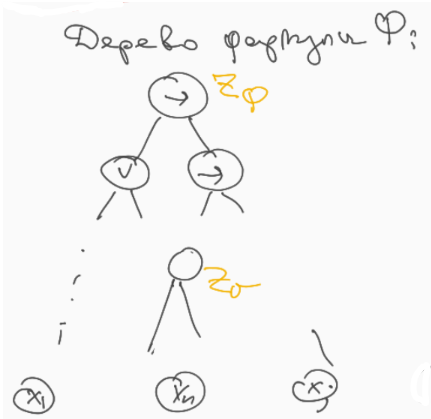
\includegraphics[width = 0.4\linewidth]{tree1.png}
\end{figure}
Заметим, что в листьях записаны переменные.\\
Вспомогательные переменные $Z_v$ ($v$- внутренняя вершина дерева).\\
Рассмотрим, как мы строим дерево:\\
\textbf{1.} $C_{\text{ф}} = Z_{\text{ф}} \underset{v \in I(t) (*)}{\bigwedge} C_v$\\
    (*)- каждая КНФ отвечает одной из внутренних вершин дерева\\
\textbf{Пример 1.1}\\
\begin{figure}[!h]
	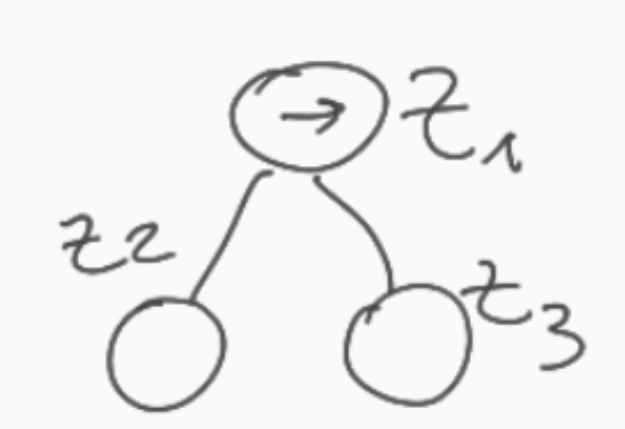
\includegraphics[width = 0.2\linewidth]{tr1.png}
\end{figure}
$C_v \equiv (Z_1 \sim (Z_2 \to Z_3))$ (членов не больше кол-ва нулей, то есть не больше 8)\\

Если вершина внутренняя, а под ней 1 или 2 вершины являются листьями (написано не $z_i$, а $x_i$), то в посылку импликации мы вставим $x_i$ вместо $z_i$. То есть будет следующий вид:

\[
C_v \equiv (Z_1 \sim (X_2 \to Z_3))\\
\]
\textbf{Пример 1.2}\\
\begin{figure}[!h]
	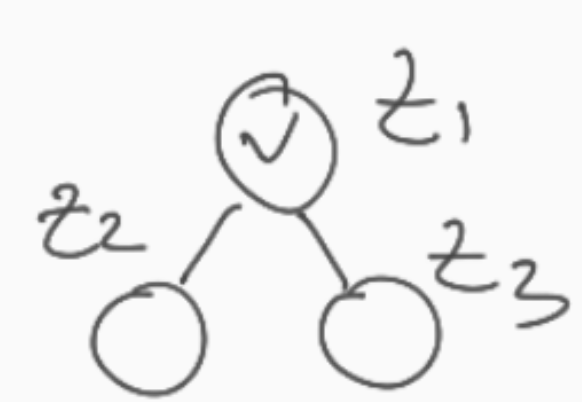
\includegraphics[width = 0.2\linewidth]{tr2.png}
\end{figure}
$C_v \equiv (Z_1 \sim (Z_2 \vee Z_3))$\\
\textbf{Пример 1.3}\\
\begin{figure}[!h]
	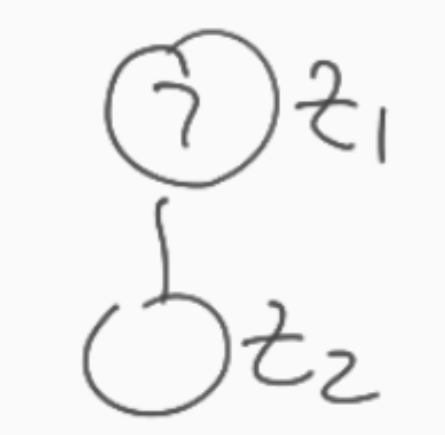
\includegraphics[width = 0.2\linewidth]{tr3.png}
\end{figure}
$C_v \equiv (Z_1 \sim \neg Z_2 )$\\
Для доказательства корректности требуется доказать следующее:
\[
\textbf{Ф(x) - выполнима $\leftrightarrow C_{\text{ф}}(x,z)$ - выполнима }
\]
\newpage
\textbf{Доказательство:}\\
\textbf{1.} Пусть выполнима Ф$(\alpha) = 1$. Рассмотрим дерево разбора формулы:\\
\bigskip
\begin{figure}[h!]
	\center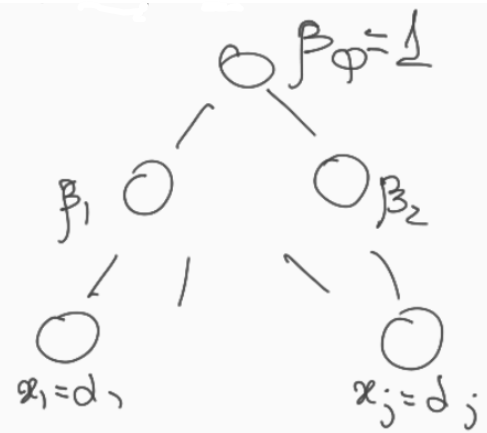
\includegraphics[width = 0.4\linewidth]{tr5.png}
\end{figure}

Припишем листьям значения $\alpha_1,...,\alpha_n$, а внутренним узлам те значения, которые возникают при вычислении по дереву $\beta_1,...,\beta_n$.\\
А затем подставим в КНФ $C_{\text{ф}}$ вместо значений $x$ и $z\Rightarrow C_{\text{ф}}(\alpha , \beta)=1 $ (тк $C_{\text{ф}} \equiv \beta_v$ вычисляется по предыдущим значениям). Следовательно, все промежуточные вершины истины и $Z_{\text{ф}}$ тоже истино, тк мы предположили, что значение формулы истино (а значит значение корня тоже истино).\\
\textbf{2.}Пусть выполнима $C_{\text{ф}}(\alpha , \beta)=1 \Rightarrow \beta_v$ задают корректные значения при вычислении по дереву формулы на наборе переменных $\alpha C_{\text{ф}}= Z_{\text{ф}} \wedge C_v $, поэтому Ф$(\alpha) = 1$.
\subsection{Задача проверки тавтологии - практичность резолюций.}
В общем виде мы имеем следующее - берется схема, состоящая из двух частей: разбора по дереву и резолюции. Запускается схема, если слишком долго, то программа останавливается, и к исходной формуле применяются эвристики и тп.\\
Во время разбора по дереву не надо подставлять все мыслимые наборы значений переменных. Мы можем, подставив значение переменной, упростить формулу.\\
\newpage
Пример (работаем с КНФ):\\
\begin{figure}[h!]
	\center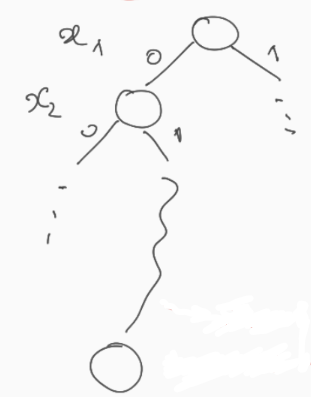
\includegraphics[width = 0.4\linewidth]{tr6.png}
\end{figure}
\newline
Берем переменную $x_1$ и присваиваем ей значение 0. Причем те дизъюнкты, куда входит $\neg x_1$ станут истинными. А в тех дизъюнктах, куда входит $ x_1$, мы можем вычеркнуть  $ x_1$, и дизъюнкт упростится. В случае, когда $x_1 = 1$, производим точно противополжные действия. И так, двигаясь по дереву, в какой-то момент может выясниться, что все оставшиеся дизъюнкты опустели, а это значит, что мы получили тождественную ложь ( не можем добиться истинности). Или же получили один дизъюнкт $ x$ , а другой $\neg x$, то мы должны остановиться и сделать рекурсивный возврат (рекурсивный перебор дерева возможностей). Еще одна возможность, что мы присвоили занчения всем переменным и никакой лжи не получилось, а значит данная ветка дает нам выполняющий набор. Следовательно, формула выполнима, и предоставляем выполняющий набор. Ну а если происходит рекурсивный возврат, мы продолжаем перебирать другую ветку.\\
\newpage
\textbf{НО} когда мы делаем рекурсивный возрат, то может быть следующая ситуация:
\begin{figure}[h!]
	\center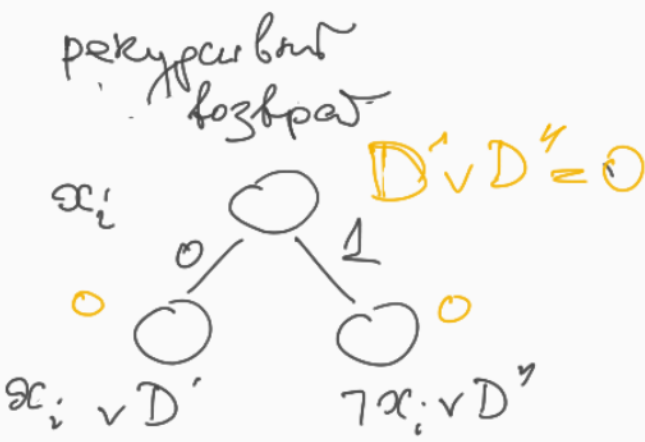
\includegraphics[width = 0.4\linewidth]{tr7.png}
\end{figure}
\newline
Предположим, что в левой нижней вершине мы нашли дизъюнкт следующего вида $x_i \vee D^{'}$, который обращается в 0 (тк $x_i=0$) , а в правой $\neg x_i \vee D^{''}$, который тоже обращается в ноль, тк есть $\neg x_i$.\\
Представим, что когда мы делаем разбор дерева то, присвоив значение 0 некоторому узлу, мы еще и указываем, какой дизъюнкт обращается в 0. \\
Очевидно, что если вернуться к реккурсивному возврату и рассмотреть, что в нижних вершинах 0, то в их предке тоже должен быть 0. Значит в данный узел по правилу резолюции мы должны вписать $D^{'}\vee D^{''}=0$, иначе бы у нас в потомках не были 0. \\
То есть применением резолюции мы можем поддерживать систему, которая устраивает частичный разбор дерева, но и поддерживает в каждом узле возврата явное указание дизъюнкта, которое следует семантически из исходных, которые обращаются в ноль. Но с помощью резолюций можно наблюдать и синтаксическое следование.\\
Получается, при каждом рекурсивном возврате мы добавляем дизъюнкт, а чем больше дизъюнктов, тем проще строить опровержение, тем больше возможностей для вывода резолюциями. Получаем самоускоряющуюся систему. \\
Данная схема позволяет справляться очень большими формулами, причем за не очень большое время.\\
\textbf{КОНЕЦ ПЕРВОЙ ЧАСТИ КУРСА!!!}











